\section{Escalamiento e Hiperparámetros}

% ================================================================
\begin{frame}{Por Qué el Escalamiento es Crítico en KNN}
\footnotesize
\begin{columns}[T,onlytextwidth]
\begin{column}{0.54\textwidth}
\begin{ccdebox}
Como KNN mide distancias absolutas en $\mathbb{R}^p$, variables con mayor escala numérica dominan arbitrariamente la cercanía.
\end{ccdebox}

\vspace{0.06cm}
\begin{itemize}\setlength{\itemsep}{0.12em}
  \item \textbf{Ejemplo}: Ingreso mensual ($\$1\,000$ a $\$20\,000$) vs. Edad ($18$ a $80$).
  \item Diferencia de $\$100$ eclipsa totalmente $40$ años de edad.
  \item \textbf{Efecto}: la distancia ignora las variables de menor escala.
\end{itemize}
\end{column}

\begin{column}{0.44\textwidth}
\centering
\begin{tikzpicture}[scale=0.72]
  \draw[->,ccdenavy,line width=0.8pt] (0,0) -- (4.0,0) node[below,font=\tiny]{Ingreso};
  \draw[->,ccdenavy,line width=0.8pt] (0,0) -- (0,3.0) node[left,font=\tiny]{Edad};
  
  % Elipse deformada amplia
  \draw[warn,thick,dashed] (2.0,1.55) ellipse (1.70cm and 0.50cm);
  \node[warn,font=\tiny\bfseries,align=center] at (2.0,2.35) {Vecindad deformada};

  % Punto de consulta x0 nítido y legible con diana
  \node (x0) at (2.0,1.55) [draw=ccdenavy,fill=white,circle,inner sep=2.4pt,line width=1.2pt] {};
  \fill[ccdenavy] (2.0,1.55) circle (1.2pt);
  \node[left=3.5pt of x0,font=\scriptsize\bfseries,text=ccdenavy] {$x_0$};

  % Puntos en la misma elipse
  \fill[ccdeaccent] (0.85,1.55) circle (2.2pt);
  \fill[ccdeaccent] (3.15,1.55) circle (2.2pt);

  % Punto descartado
  \fill[purplex] (2.0,0.50) circle (2.2pt) node (pout) {};
  \node[right=2.5pt of pout,font=\tiny,text=purplex,align=left]{Descartado a pesar\\de ser cercano};
\end{tikzpicture}

\vspace{0.08cm}
\begin{contrastbox}{okgreen}{Solución con StandardScaler}
Estandarizar ($z = \frac{x - \mu}{\sigma}$) en un \texttt{Pipeline} para evitar fuga de datos (\textit{leakage}).
\end{contrastbox}
\end{column}
\end{columns}
\source{Géron (2022), cap. 3; James et al. (2013), cap. 4.}
\end{frame}

% ================================================================
\begin{frame}{El Papel de $k$: Trade-Off Sesgo--Varianza}
\begin{columns}[T,onlytextwidth]
\begin{column}{0.48\textwidth}
\begin{contrastbox}{warn}{k Pequeño: Flexibilidad}
\scriptsize
\textbf{Bajo sesgo / Alta varianza ($k=1$)}
\begin{itemize}\setlength{\itemsep}{0.10em}
  \item Reproduce fielmente el training set.
  \item Frontera fragmentada, sensible a anomalías.
\end{itemize}
\end{contrastbox}

\vspace{0.08cm}
\begin{contrastbox}{ccdemid}{k Grande: Regularización}
\scriptsize
\textbf{Alto sesgo / Baja varianza ($k \to N$)}
\begin{itemize}\setlength{\itemsep}{0.10em}
  \item Fronteras excesivamente suaves.
  \item Predice la clase mayoritaria global.
\end{itemize}
\end{contrastbox}
\end{column}

\begin{column}{0.49\textwidth}
\centering
\begin{tikzpicture}[scale=0.74]
  \draw[->,ccdenavy,line width=0.8pt] (0,0) -- (4.2,0) node[right,font=\tiny]{$1/k$};
  \draw[->,ccdenavy,line width=0.8pt] (0,0) -- (0,2.9) node[left,font=\tiny]{Error};

  \draw[okgreen,thick] (0.4,2.3) to[out=-40,in=175] (3.8,0.3);
  \node[okgreen,font=\tiny\bfseries] at (3.8,0.55) {Train};

  \draw[warn,thick] (0.4,2.5) to[out=-50,in=180] (2.0,1.1) to[out=0,in=215] (3.8,2.4);
  \node[warn,font=\tiny\bfseries] at (3.8,2.65) {Test};

  \draw[ccdemid,dashed,line width=0.8pt] (2.0,0) -- (2.0,1.1);
  \node[below=1pt,font=\tiny\bfseries,text=ccdemid] at (2.0,0) {$k^*$ óptimo};
  \fill[ccdemid] (2.0,1.1) circle (2pt);
\end{tikzpicture}

\vspace{0.06cm}
\begin{keybox}
\footnotesize \textbf{Regla}: el hiperparámetro $k$ se optimiza mediante \textbf{validación cruzada} (CV).
\end{keybox}
\end{column}
\end{columns}
\source{Hastie, Tibshirani \& Friedman (2009), cap. 2 y 13.}
\end{frame}

% ================================================================
\begin{frame}{Evolución de las Regiones de Decisión según $k$}
\centering
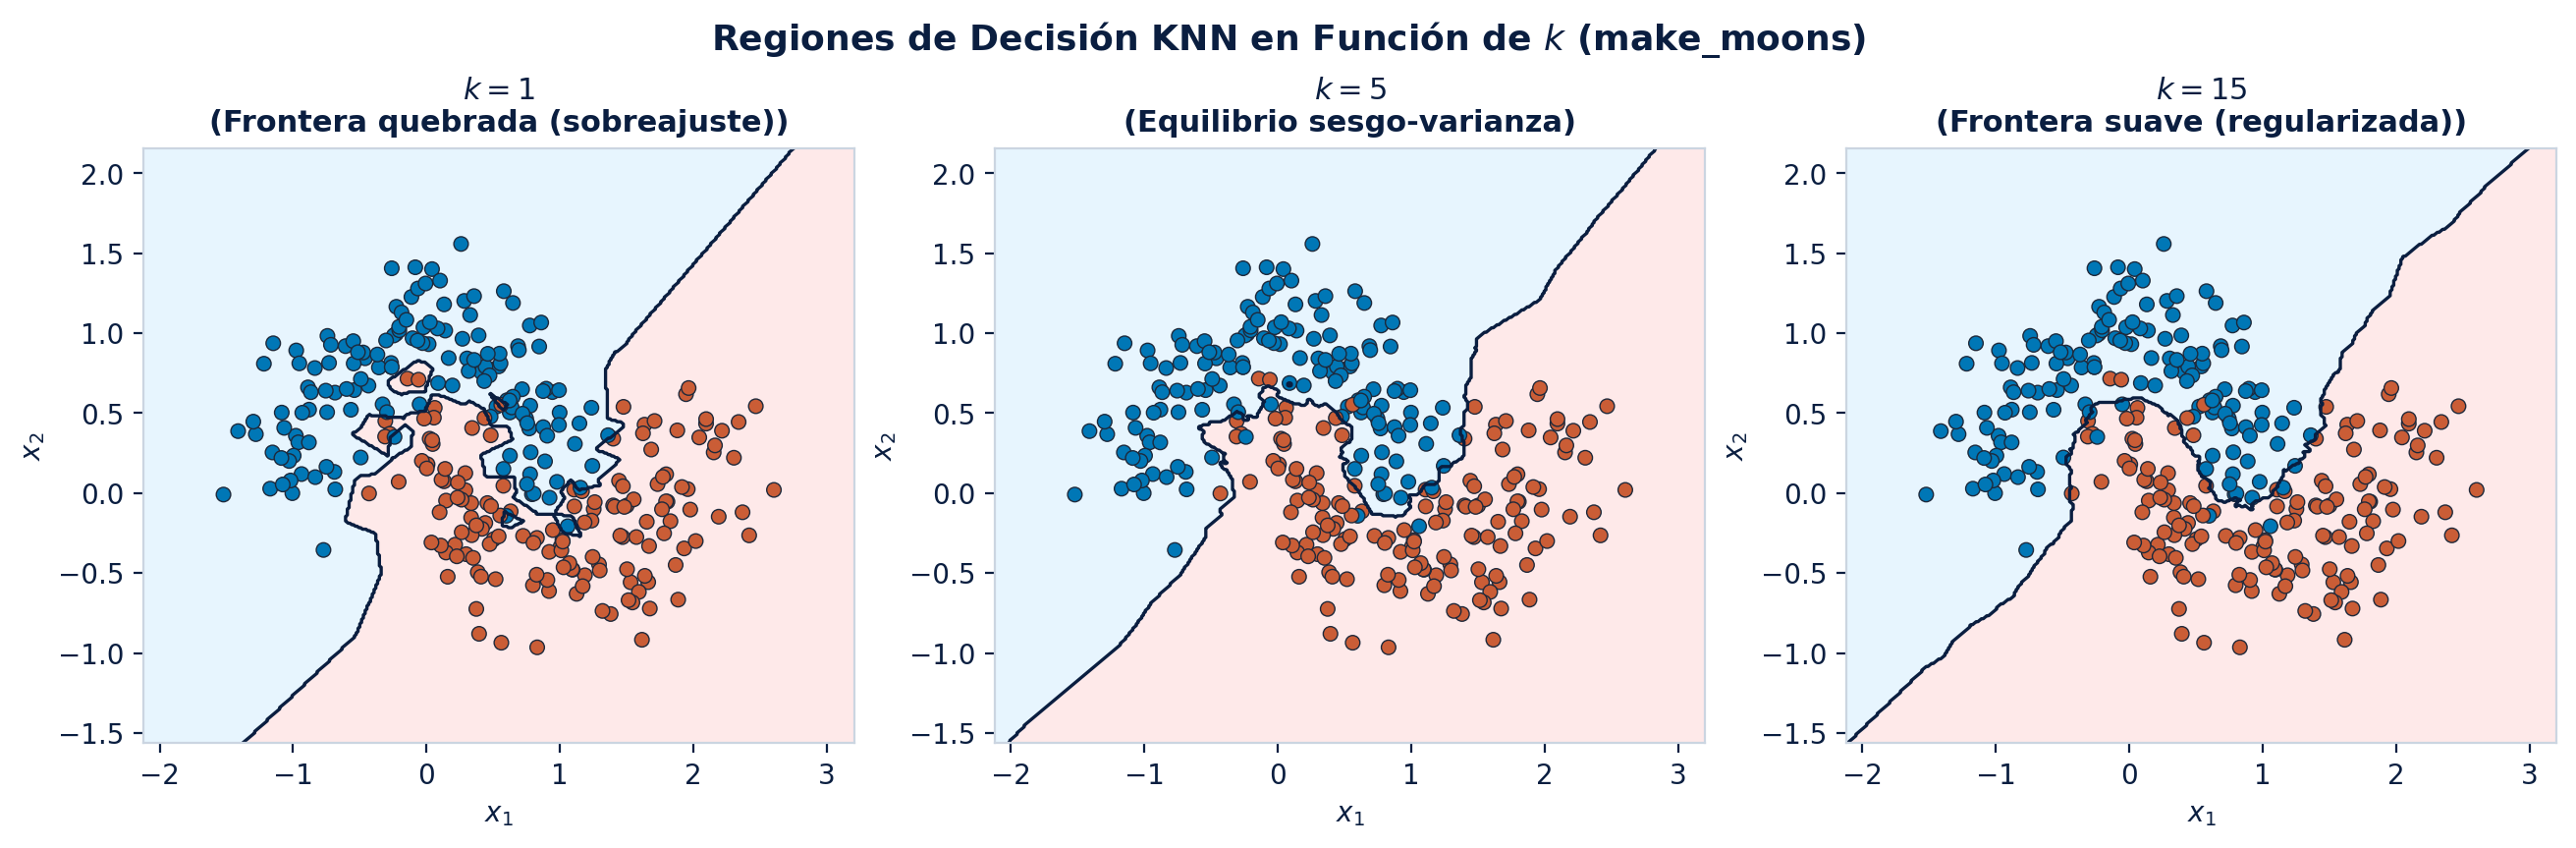
\includegraphics[width=0.90\linewidth]{fig_knn_regions.png}

\vspace{-0.05cm}
\begin{columns}[T,onlytextwidth]
\begin{column}{0.32\textwidth}
\begin{ccdebox}
\scriptsize
\textbf{$k = 1$ (Sobreajuste):}\\
Frontera hiperflexible; islas espurias alrededor de puntos ruidosos.
\end{ccdebox}
\end{column}

\begin{column}{0.32\textwidth}
\begin{keybox}
\scriptsize
\textbf{$k = 5$ (Balance Óptimo):}\\
Captura la curvatura no lineal de las lunas respetando la estructura.
\end{keybox}
\end{column}

\begin{column}{0.32\textwidth}
\begin{ccdebox}
\scriptsize
\textbf{$k = 15$ (Regularizado):}\\
Frontera suave y estable; reduce la varianza minimizando el sobreajuste.
\end{ccdebox}
\end{column}
\end{columns}
\source{Figura generada con scikit-learn (\texttt{make\_moons}) y \texttt{KNeighborsClassifier}.}
\end{frame}
